\section{short project}
\subsection{a}
Use algorithm 4.2 of Curtis's book for calculation.

$$
v_r = \dfrac{\boldsymbol r \boldsymbol v}{r} =  0.0102 ~km /\sec \to \text{away from perigee}
$$

$$
\boldsymbol h = \boldsymbol r \boldsymbol v = \begin{bmatrix}
    11368 &  -31882  &  39764
\end{bmatrix}
$$
$$
\boldsymbol e = \dfrac{\boldsymbol v \times \boldsymbol h}{\mu} - \dfrac{\boldsymbol r}{r}
$$
Others Parameters have been calculated in short\_project/short\_project.m



\begin{center}
    \begin{longtable}{|c|c|c|c|c|c|c|c|c|}
        \caption{The position and velocity components and magnitude with time for $\Delta t = 100 \sec$.}\\
    
    \hline \multicolumn{1}{|c|}{\textbf{Time (s)}} &
    \multicolumn{3}{c|}{\textbf{Position}} &
    \multicolumn{1}{c|}{\textbf{Pos magnitude}} &
    \multicolumn{3}{c|}{\textbf{Velocity}} &
    \multicolumn{1}{c|}{\textbf{magnitude}}  \\ \hline 
    \endfirsthead
    
    \multicolumn{9}{c}%
    {{\bfseries \tablename\ \thetable{} -- continued from previous page}} \\
    \hline \multicolumn{1}{|c|}{\textbf{Time (s)}} &
    \multicolumn{3}{c|}{\textbf{Position}} &
    \multicolumn{1}{c|}{\textbf{magnitude}} &
    \multicolumn{3}{c|}{\textbf{Velocity}} &
    \multicolumn{1}{c|}{\textbf{magnitude}} \\ \hline 
    \endhead
    
    \hline \multicolumn{9}{|r|}{{Continued on next page}} \\ \hline
    \endfoot
    
    \hline
    \endlastfoot
    65.57 & 1600.00 & 5310.00 & 3800.00  & 6722.80 & -7.35 &  0.46 &  2.47 & 7.77 \\ 
    165.57 & 856.12 & 5321.11 & 4021.57  & 6724.60 & -7.51 &  -0.24 &  1.96 & 7.77 \\ 
    265.57 & 101.01 & 5262.55 & 4190.48  & 6727.90 & -7.57 &  -0.93 &  1.42 & 7.76 \\ 
    365.57 & -655.39 & 5135.19 & 4304.60  & 6732.70 & -7.54 &  -1.61 &  0.86 & 7.76 \\ 
    465.57 & -1403.24 & 4940.84 & 4362.57  & 6738.91 & -7.40 &  -2.27 &  0.30 & 7.75 \\ 
    565.57 & -2132.91 & 4682.10 & 4363.72  & 6746.36 & -7.17 &  -2.90 &  -0.27 & 7.74 \\ 
    665.57 & -2834.92 & 4362.59 & 4308.23  & 6754.99 & -6.85 &  -3.48 &  -0.83 & 7.73 \\ 
    765.57 & -3500.22 & 3986.83 & 4197.15  & 6764.79 & -6.44 &  -4.02 &  -1.38 & 7.72 \\ 
    865.57 & -4120.41 & 3559.88 & 4032.13  & 6775.59 & -5.95 &  -4.51 &  -1.91 & 7.71 \\ 
    965.57 & -4687.82 & 3087.35 & 3815.48  & 6787.14 & -5.39 &  -4.93 &  -2.42 & 7.69 \\ 
    1065.57 & -5195.49 & 2575.36 & 3550.11  & 6799.18 & -4.76 &  -5.29 &  -2.89 & 7.68 \\ 
    1165.57 & -5637.30 & 2030.58 & 3239.63  & 6811.58 & -4.07 &  -5.59 &  -3.32 & 7.67 \\ 
    1265.57 & -6008.06 & 1460.29 & 2888.38  & 6824.36 & -3.34 &  -5.81 &  -3.70 & 7.65 \\ 
    1365.57 & -6303.53 & 871.83 & 2501.03  & 6837.38 & -2.57 &  -5.95 &  -4.04 & 7.64 \\ 
    1465.57 & -6520.44 & 272.58 & 2082.58  & 6850.37 & -1.77 &  -6.02 &  -4.32 & 7.62 \\ 
    1565.57 & -6656.50 & -330.08 & 1638.28  & 6863.08 & -0.95 &  -6.02 &  -4.55 & 7.61 \\ 
    1665.57 & -6710.39 & -928.79 & 1173.66  & 6875.28 & -0.13 &  -5.94 &  -4.73 & 7.59 \\ 
    1765.57 & -6681.99 & -1516.15 & 694.61  & 6886.96 & 0.69 &  -5.79 &  -4.84 & 7.58 \\ 
    1865.57 & -6572.19 & -2084.95 & 207.18  & 6898.08 & 1.50 &  -5.57 &  -4.90 & 7.57 \\ 
    1965.57 & -6382.70 & -2628.35 & -282.68  & 6908.48 & 2.29 &  -5.29 &  -4.89 & 7.56 \\ 
    2065.57 & -6116.11 & -3139.98 & -769.09  & 6917.93 & 3.04 &  -4.94 &  -4.83 & 7.55 \\ 
    2165.57 & -5775.82 & -3613.83 & -1246.29  & 6926.26 & 3.76 &  -4.53 &  -4.71 & 7.54 \\ 
    2265.57 & -5366.09 & -4044.38 & -1708.63  & 6933.35 & 4.43 &  -4.07 &  -4.53 & 7.53 \\ 
    2365.57 & -4892.26 & -4426.58 & -2150.52  & 6939.28 & 5.04 &  -3.57 &  -4.30 & 7.52 \\ 
    2465.57 & -4360.25 & -4755.99 & -2566.72  & 6944.01 & 5.59 &  -3.02 &  -4.02 & 7.52 \\ 
    2565.57 & -3776.47 & -5028.79 & -2952.34  & 6947.43 & 6.08 &  -2.43 &  -3.69 & 7.51 \\ 
    2665.57 & -3147.81 & -5241.84 & -3302.87  & 6949.43 & 6.49 &  -1.82 &  -3.32 & 7.51 \\ 
    2765.57 & -2481.63 & -5392.61 & -3614.20  & 6949.91 & 6.82 &  -1.19 &  -2.90 & 7.51 \\ 
    2865.57 & -1785.89 & -5479.34 & -3882.63  & 6948.91 & 7.08 &  -0.54 &  -2.46 & 7.51 \\ 
    2965.57 & -1069.05 & -5501.04 & -4104.96  & 6946.59 & 7.25 &  0.11 &  -1.98 & 7.51 \\ 
    3065.57 & -339.66 & -5457.43 & -4278.50  & 6942.94 & 7.33 &  0.76 &  -1.48 & 7.52 \\ 
    3165.57 & 393.70 & -5348.88 & -4401.13  & 6937.97 & 7.33 &  1.41 &  -0.97 & 7.52 \\ 
    3265.57 & 1122.40 & -5176.49 & -4471.22  & 6931.64 & 7.23 &  2.04 &  -0.43 & 7.53 \\ 
    3365.57 & 1837.79 & -4942.03 & -4487.76  & 6923.96 & 7.06 &  2.65 &  0.10 & 7.54 \\ 
    3465.57 & 2531.12 & -4648.26 & -4450.42  & 6915.13 & 6.79 &  3.22 &  0.64 & 7.55 \\ 
    3565.57 & 3193.84 & -4298.58 & -4359.52  & 6905.35 & 6.45 &  3.76 &  1.17 & 7.56 \\ 
    3665.57 & 3817.85 & -3897.02 & -4215.94  & 6894.70 & 6.02 &  4.26 &  1.70 & 7.57 \\ 
    3765.57 & 4395.43 & -3448.11 & -4021.14  & 6883.23 & 5.52 &  4.71 &  2.20 & 7.58 \\ 
    3865.57 & 4919.32 & -2956.99 & -3777.14  & 6870.97 & 4.95 &  5.10 &  2.68 & 7.59 \\ 
    3965.57 & 5382.78 & -2429.41 & -3486.64  & 6858.06 & 4.31 &  5.44 &  3.13 & 7.61 \\ 
    4065.57 & 5779.73 & -1871.92 & -3153.13  & 6844.82 & 3.62 &  5.70 &  3.54 & 7.62 \\ 
    4165.57 & 6104.87 & -1291.31 & -2780.57  & 6831.43 & 2.88 &  5.90 &  3.91 & 7.64 \\ 
    4265.57 & 6353.76 & -694.67 & -2373.35  & 6818.04 & 2.09 &  6.02 &  4.23 & 7.65 \\ 
    4365.57 & 6522.78 & -89.28 & -1936.29  & 6804.69 & 1.28 &  6.07 &  4.50 & 7.67 \\ 
    4465.57 & 6609.19 & 517.33 & -1474.62  & 6791.44 & 0.45 &  6.05 &  4.72 & 7.68 \\ 
    4565.57 & 6611.49 & 1117.39 & -994.18  & 6778.55 & -0.40 &  5.94 &  4.88 & 7.70 \\ 
    4665.57 & 6529.30 & 1703.04 & -501.12  & 6766.33 & -1.24 &  5.76 &  4.97 & 7.71 \\ 
    4765.57 & 6363.28 & 2266.70 & -1.73  & 6754.95 & -2.08 &  5.50 &  5.01 & 7.72 \\ 
    4865.57 & 6115.09 & 2801.05 & 497.64  & 6744.47 & -2.89 &  5.17 &  4.97 & 7.73 \\ 
    4965.57 & 5787.40 & 3299.02 & 990.58  & 6734.89 & -3.66 &  4.78 &  4.88 & 7.74 \\ 
    5065.57 & 5384.01 & 3753.97 & 1470.66  & 6726.26 & -4.39 &  4.31 &  4.71 & 7.75 \\ 
    5165.57 & 4910.19 & 4159.74 & 1931.45  & 6718.92 & -5.07 &  3.79 &  4.49 & 7.76 \\ 
    5265.57 & 4372.08 & 4510.86 & 2366.80  & 6713.02 & -5.68 &  3.22 &  4.21 & 7.77 \\ 
    5365.57 & 3776.56 & 4802.60 & 2770.96  & 6708.62 & -6.22 &  2.61 &  3.87 & 7.77 \\ 
    5465.57 & 3131.21 & 5030.98 & 3138.55  & 6705.65 & -6.68 &  1.95 &  3.48 & 7.78 \\ 
    5565.57 & 2444.39 & 5192.81 & 3464.65  & 6704.03 & -7.05 &  1.28 &  3.04 & 7.78 \\ 
    5665.57 & 1725.27 & 5286.00 & 3744.95  & 6703.95 & -7.32 &  0.58 &  2.56 & 7.78 \\ 
   
    \end{longtable}
    \end{center}

    \subsection{part b}

    \begin{figure}[H]
        \caption{3D trajectory}
        \centering
        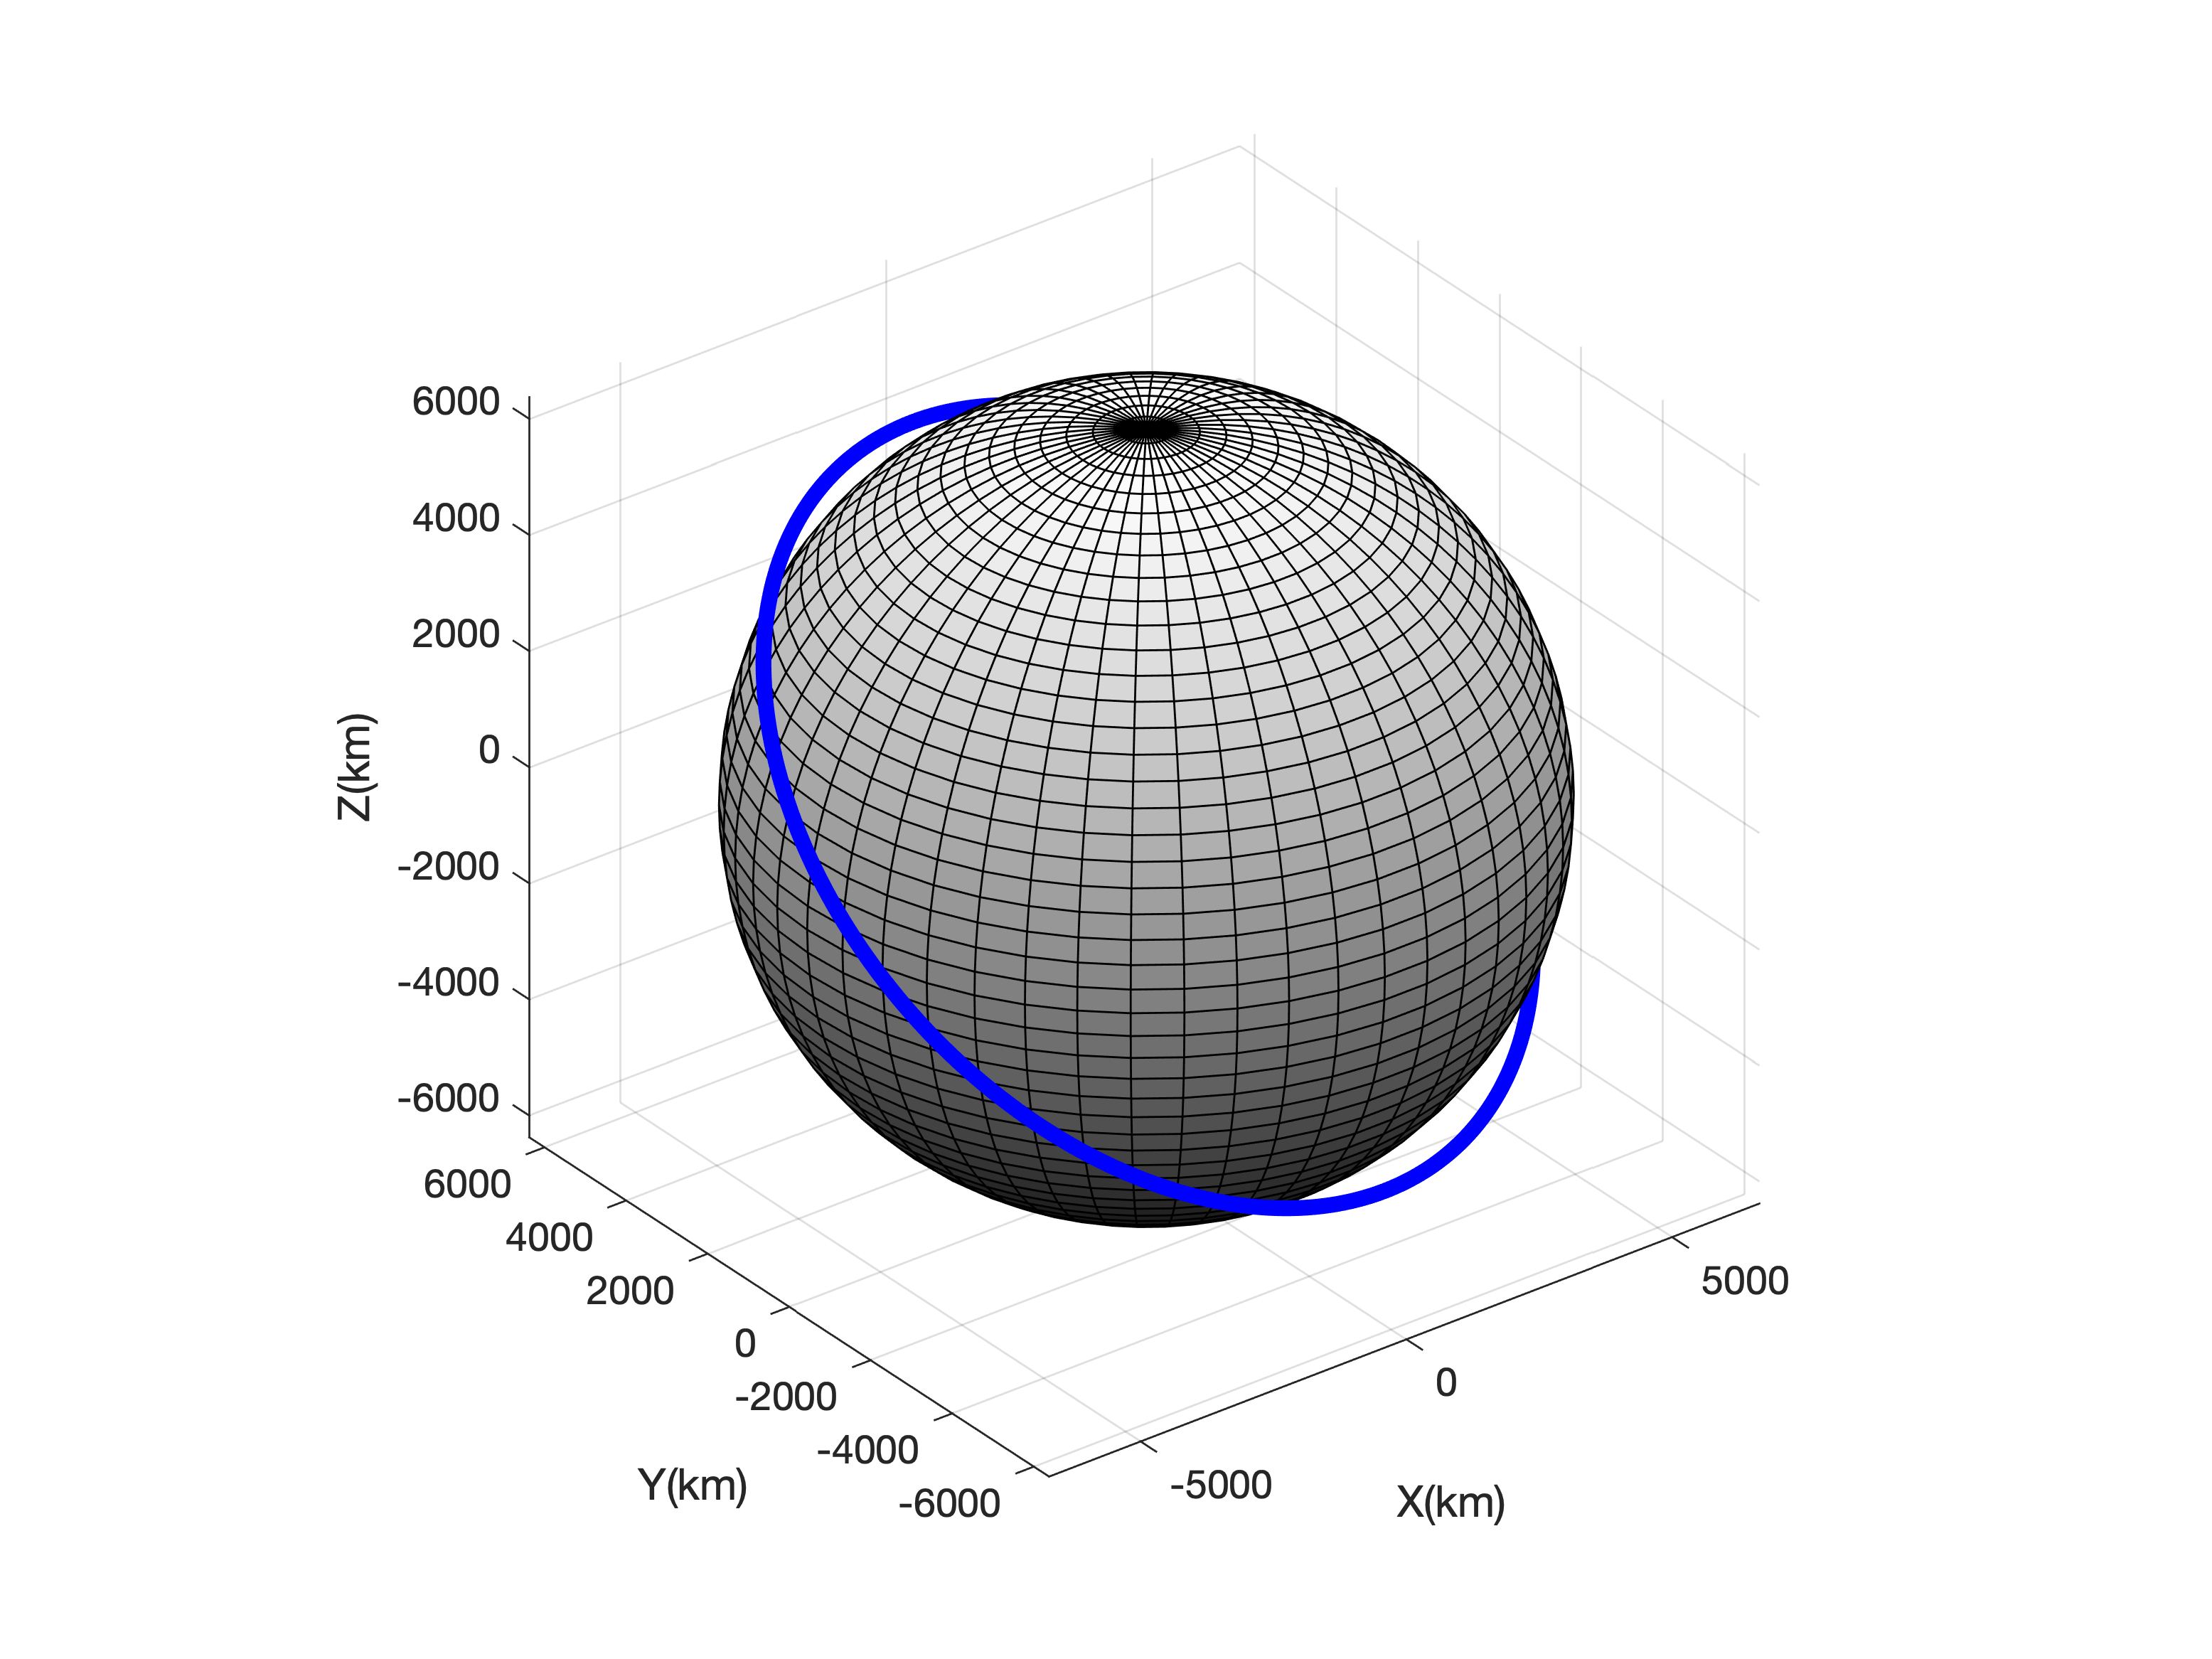
\includegraphics[width=16cm]{../Figure/Short_project/3Dof_view.png}
    \end{figure}

    \begin{figure}[H]
        \caption{3D trajectory in zx axis}
        \centering
        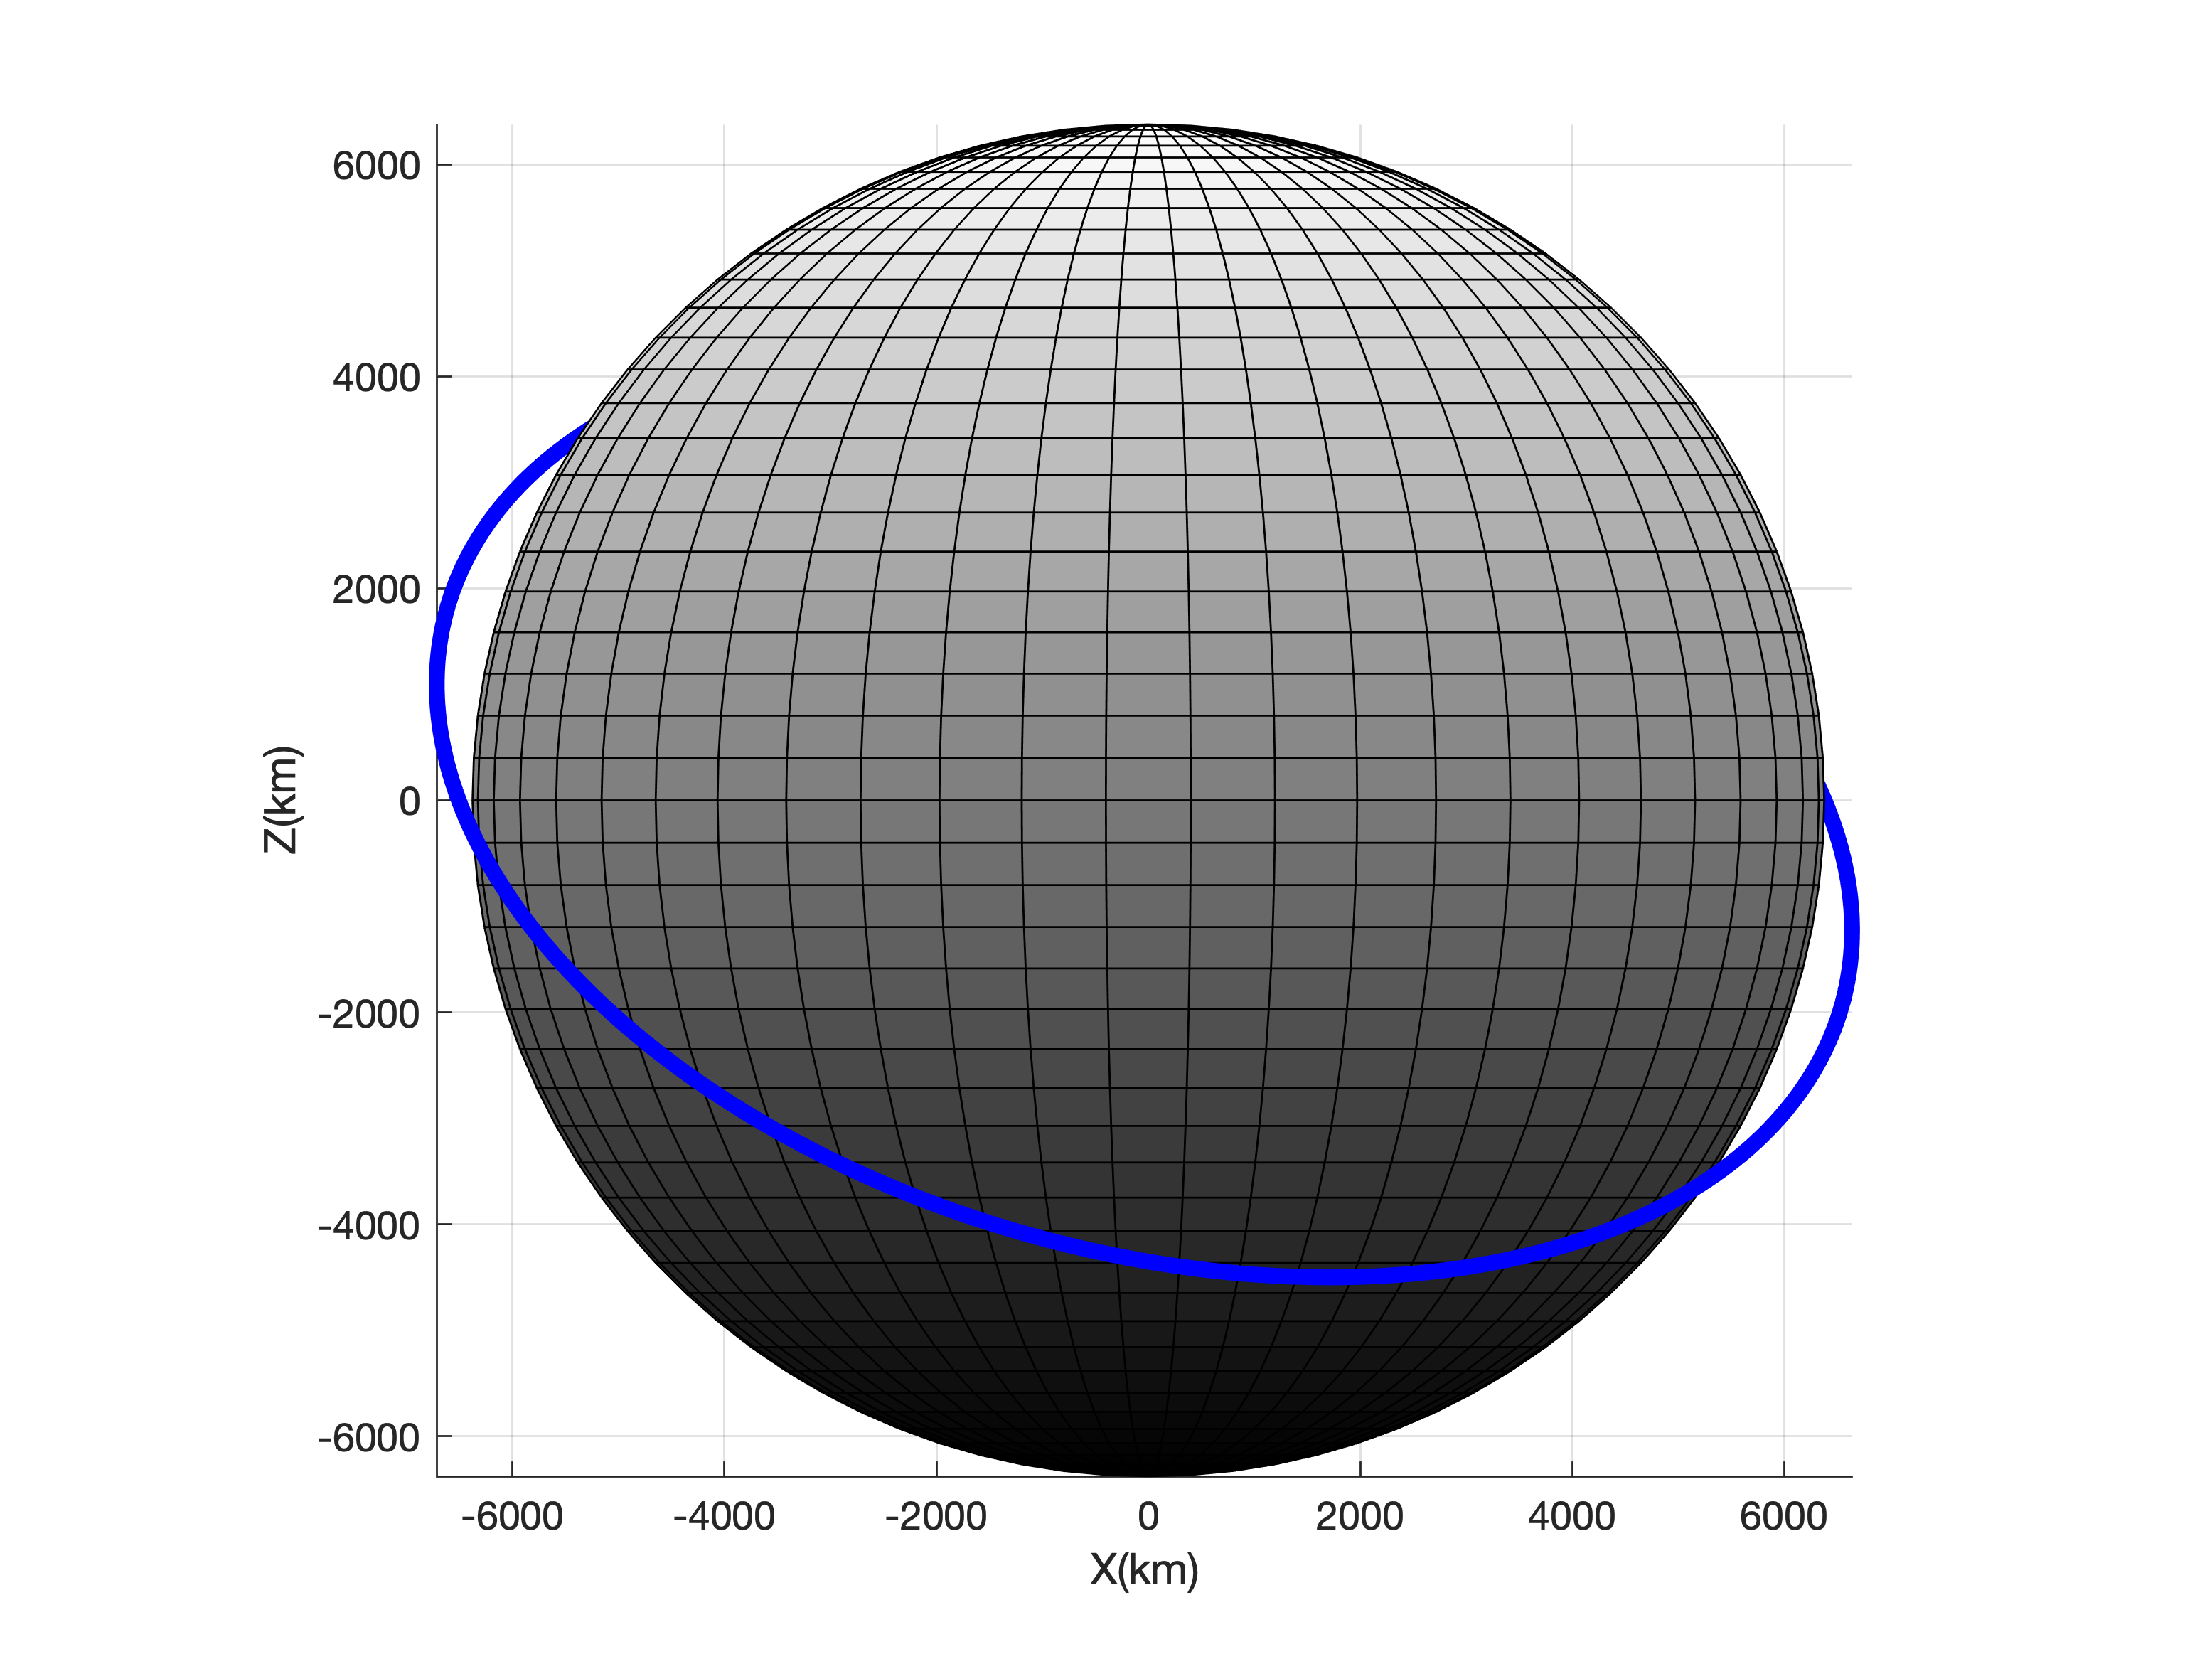
\includegraphics[width=16cm]{../Figure/Short_project/xz_view.png}
    \end{figure}

    \begin{figure}[H]
        \caption{3D trajectory in zy axis}
        \centering
        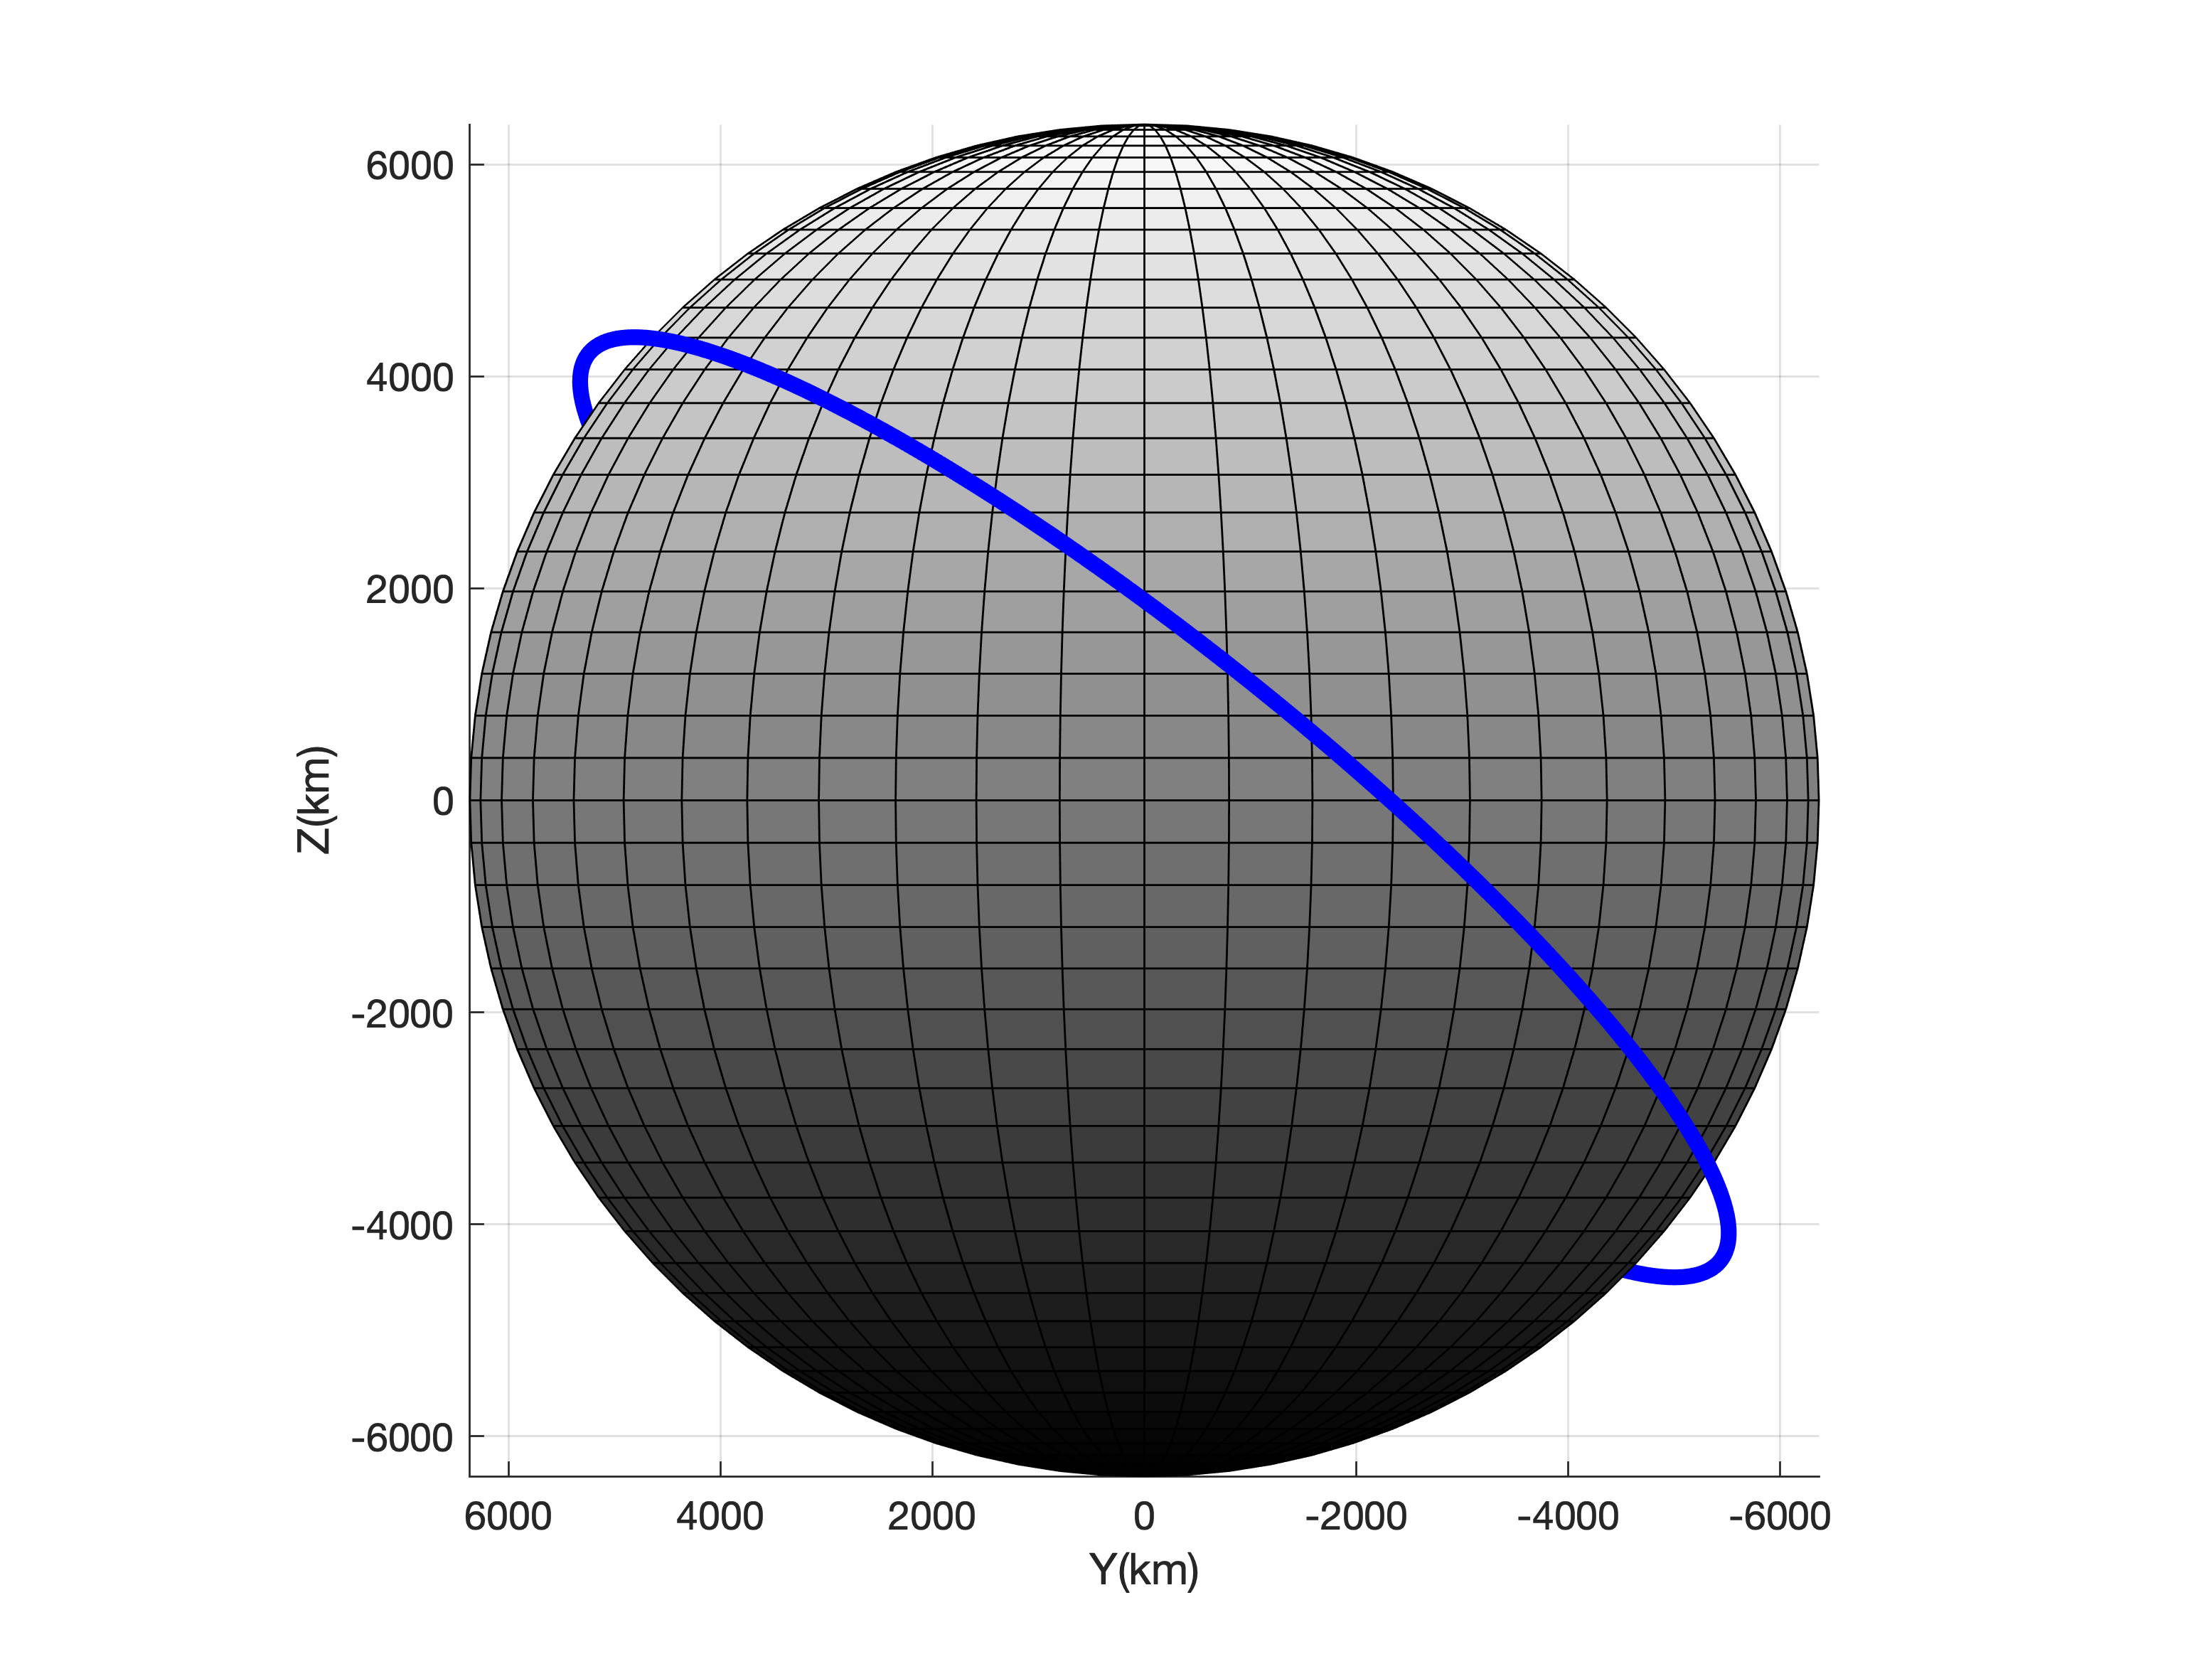
\includegraphics[width=16cm]{../Figure/Short_project/yz_view.png}
    \end{figure}

    \begin{figure}[H]
        \caption{3D trajectory in xy axis}
        \centering
        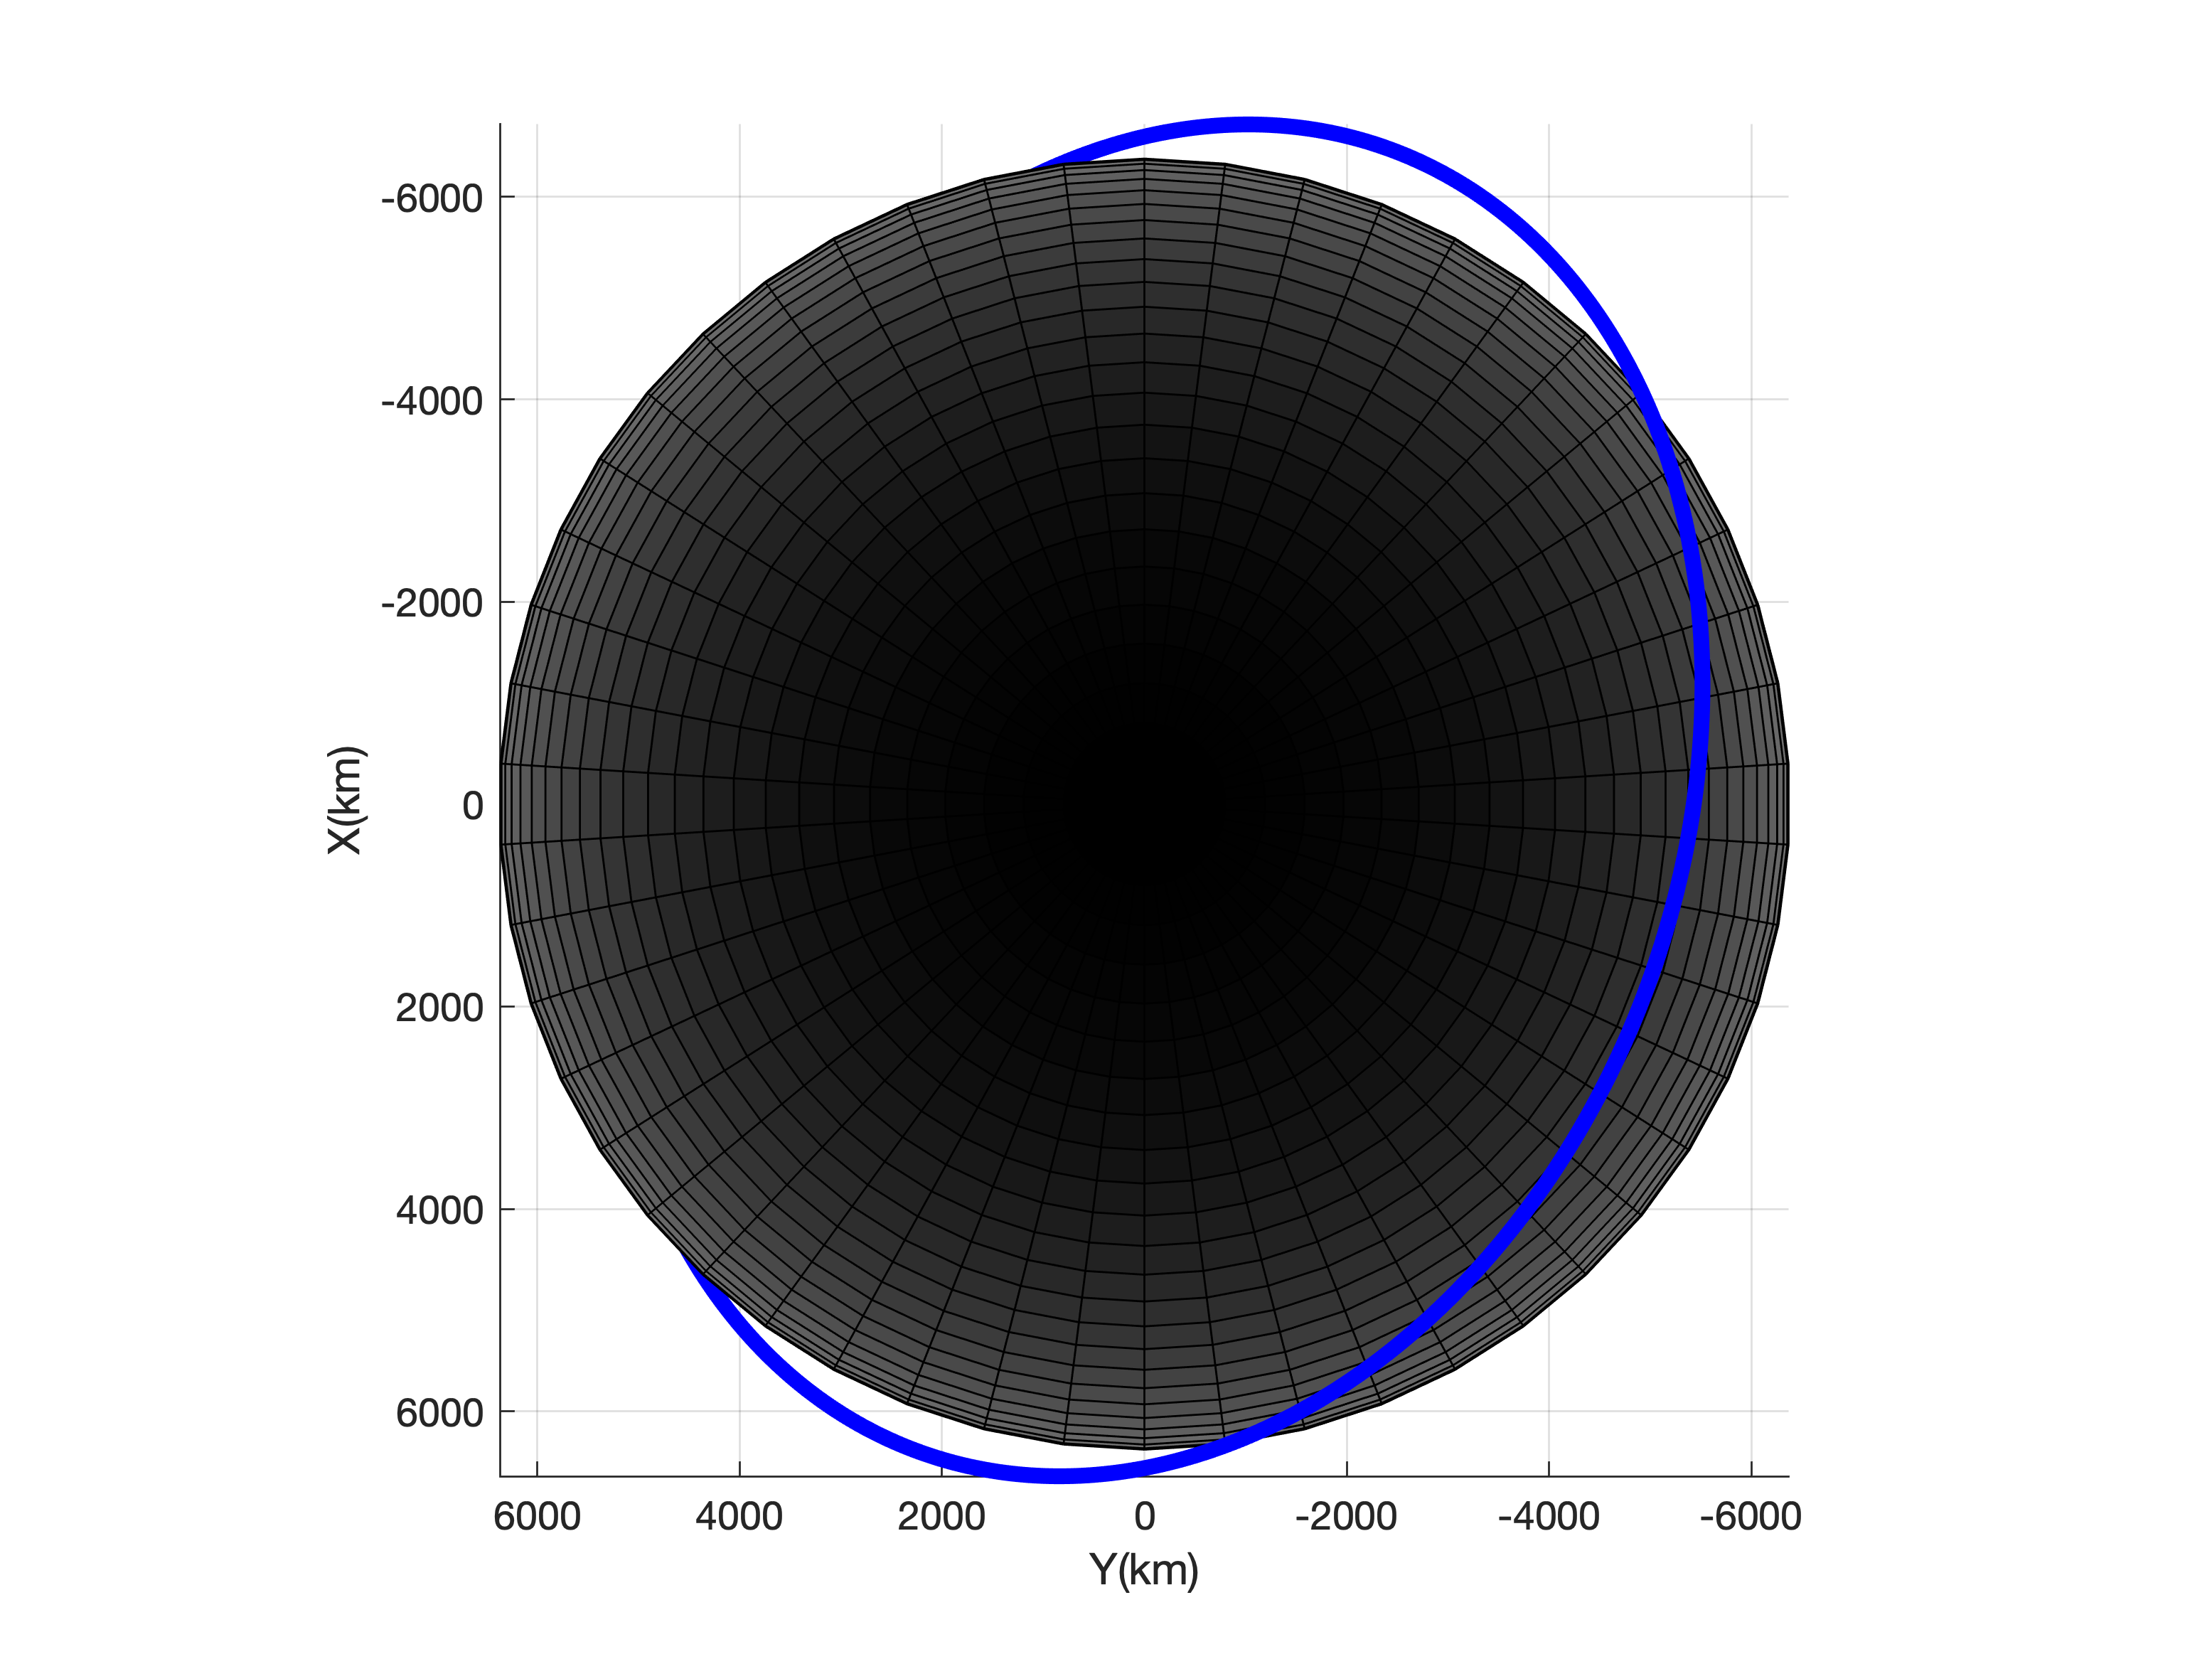
\includegraphics[width=16cm]{../Figure/Short_project/xy_view.png}
    \end{figure}

    \subsection{part c}
    Using below tranfer matrix to tranfer from ECI corrdinate to ECEF corrdinate.
    $$
    \boldsymbol T^{ECCF-ECI} = \begin{bmatrix}
        \cos(\omega_Et) & -\sin(\omega_Et)& 0\\
        \sin(\omega_Et) &  \cos(\omega_Et)& 0\\
                0       &      0          & 1
    \end{bmatrix}
    $$

    $$
    \phi = \arccos(\dfrac{\boldsymbol r(3)}{r})
    $$

    $$
    \lambda = 
\begin{cases}
    \arctan(\dfrac{\boldsymbol r(1)}{r_{xy}}),& \boldsymbol r(2) > 0\\
    2\pi-\arctan(\dfrac{\boldsymbol r(1)}{r_{xy}}),& \boldsymbol r(2) \leq 0\\
\end{cases}
    $$

    \begin{figure}[H]
        \caption{Satellite latitude versus its longitude for one period}
        \centering
        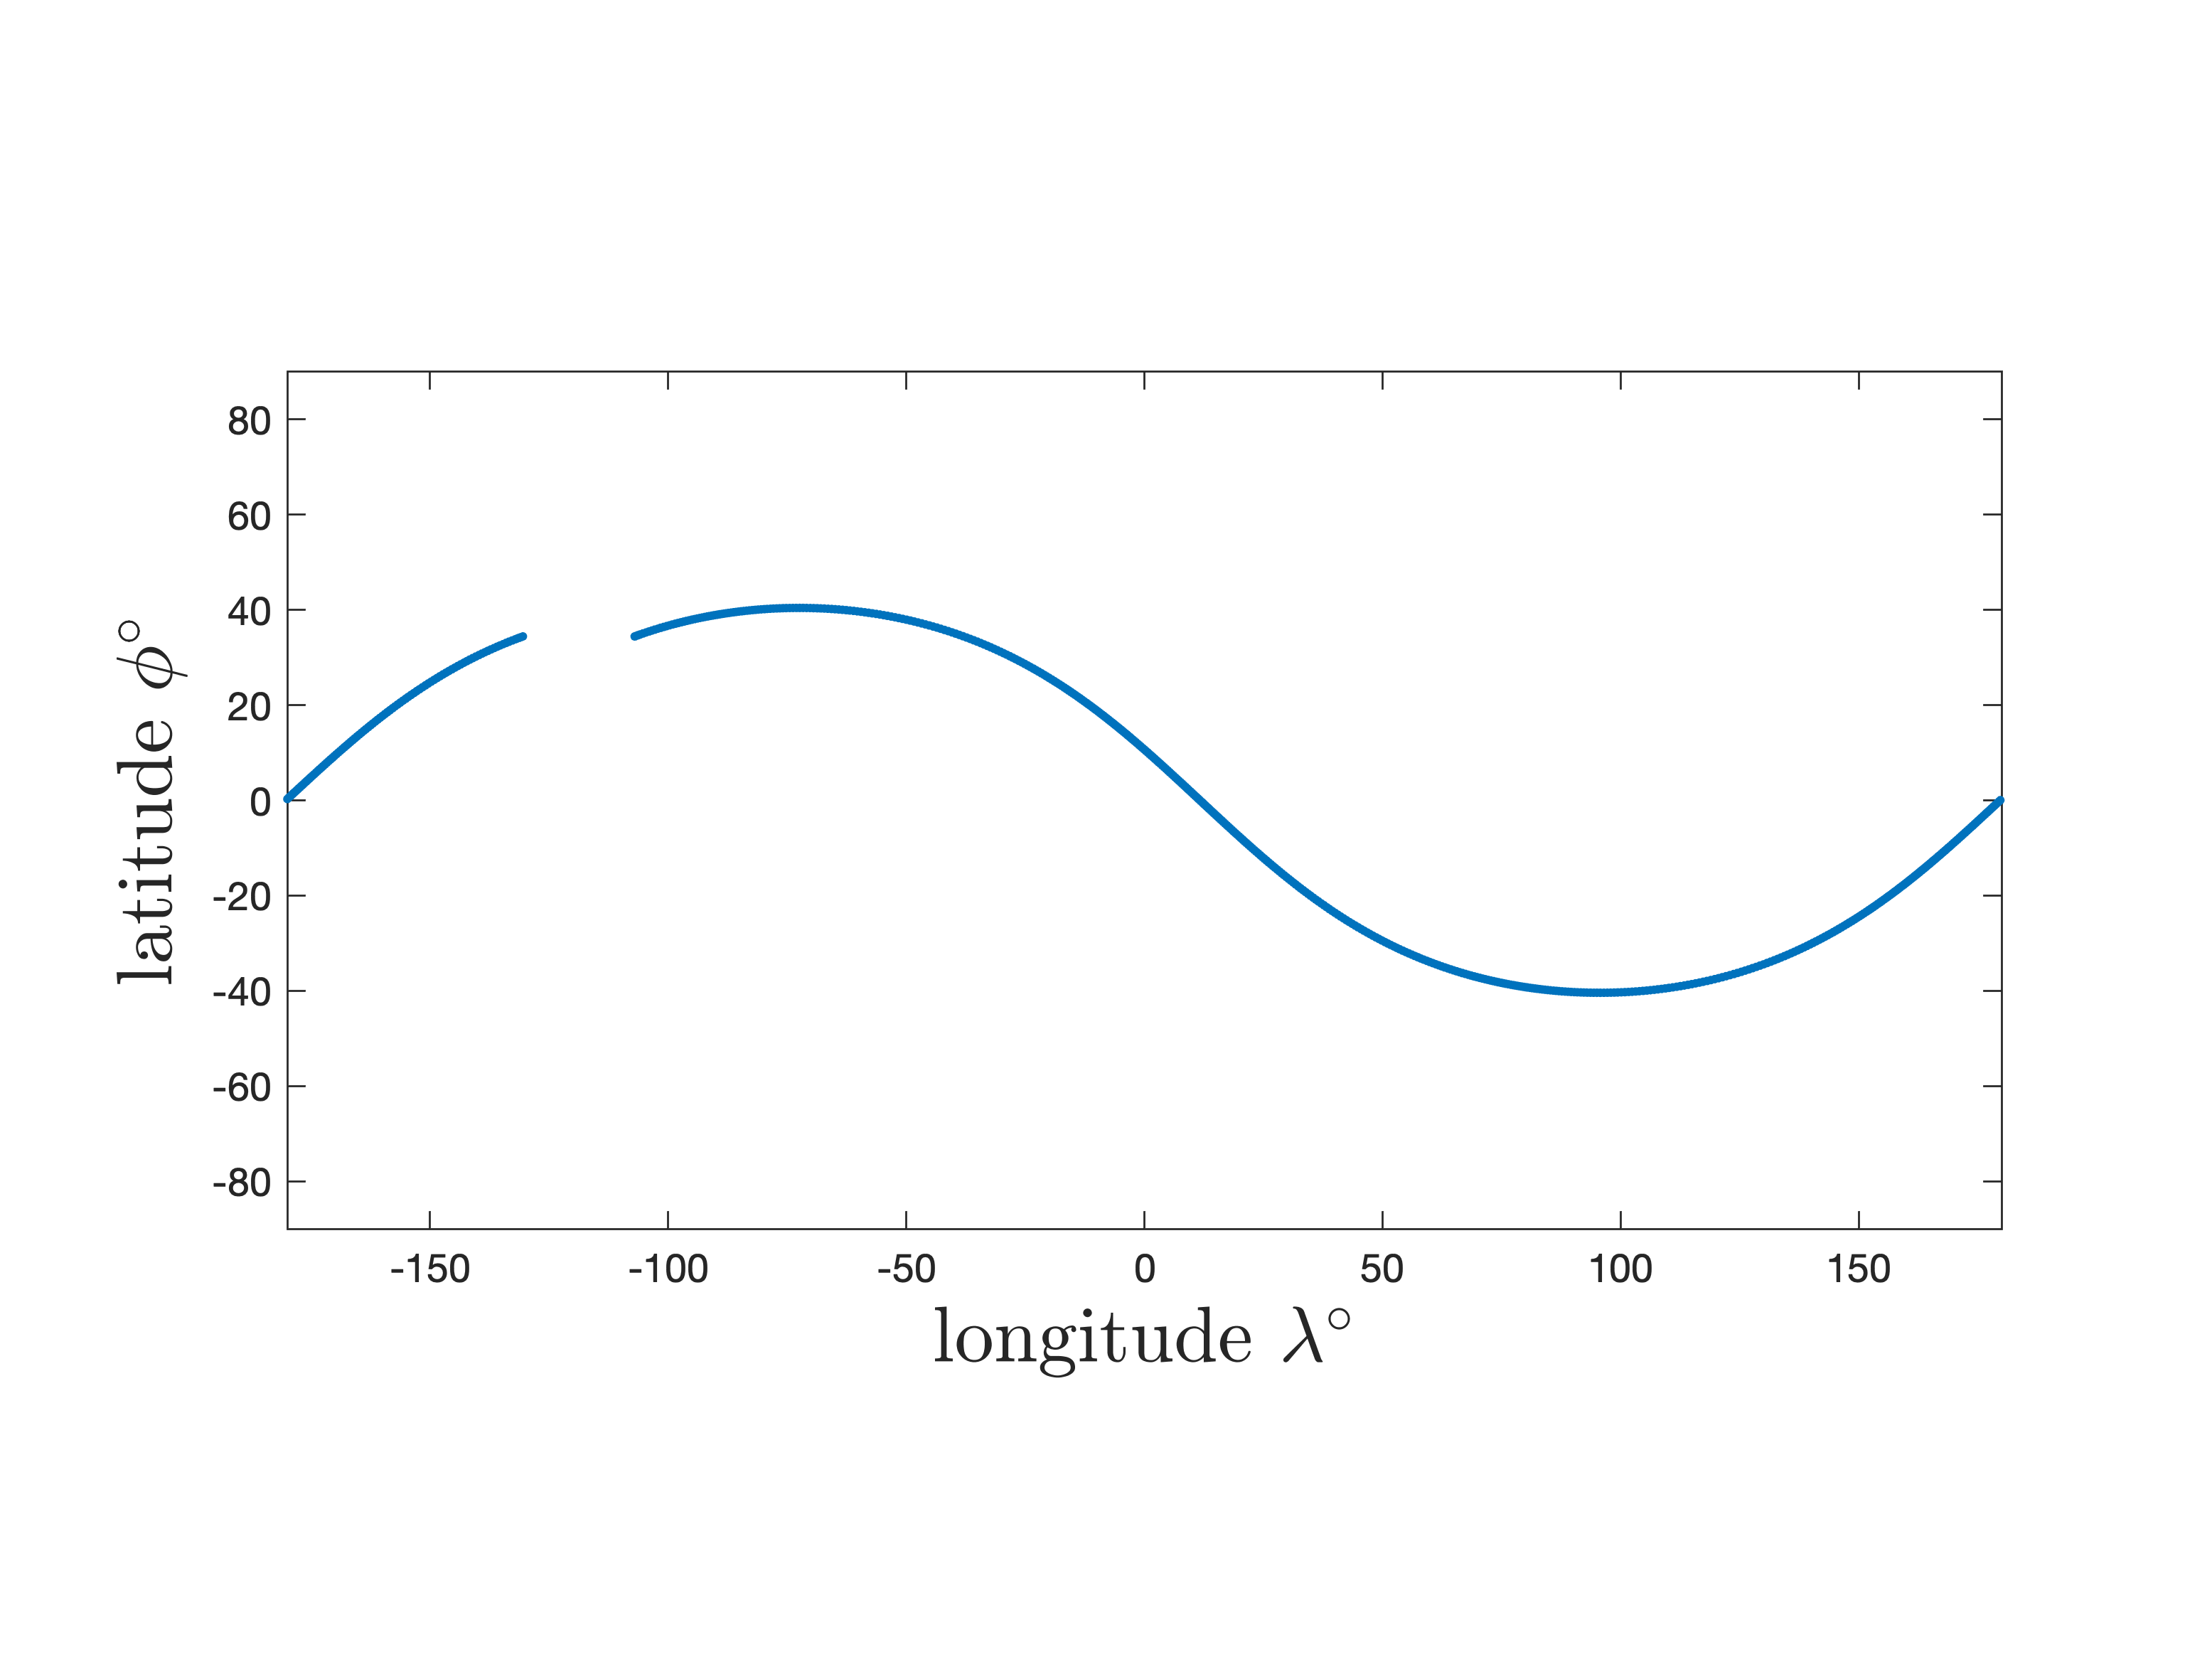
\includegraphics[width=16cm]{../Figure/Short_project/latlong.png}
    \end{figure}

    Below the figure drawn provided by tamaskis, please click \href{https://github.com/tamaskis/ground_track-MATLAB}{here} to see the source code. Please use mentioned library to run code or skip part on earth fig.

    \begin{figure}[H]
        \caption{Satellite latitude versus its longitude for one period}
        \centering
        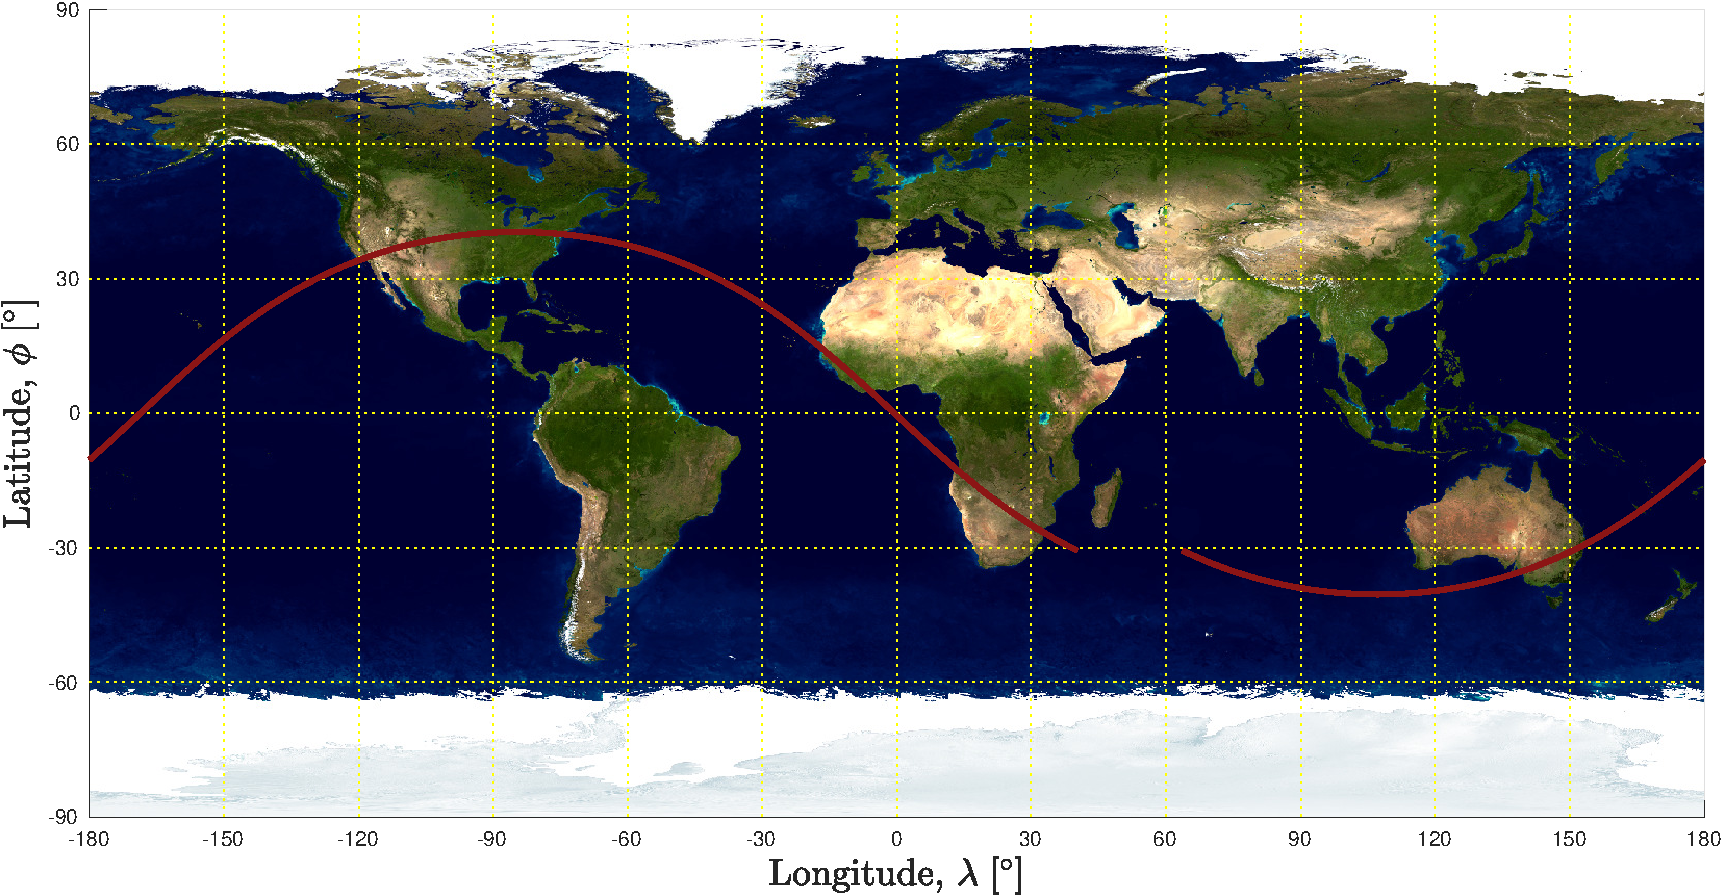
\includegraphics[width=16cm]{../Figure/Short_project/latlong_earth.png}
    \end{figure}

